% Options for packages loaded elsewhere
\PassOptionsToPackage{unicode}{hyperref}
\PassOptionsToPackage{hyphens}{url}
%
\documentclass[
  12pt,
]{article}
\usepackage{amsmath,amssymb}
\usepackage{lmodern}
\usepackage{ifxetex,ifluatex}
\ifnum 0\ifxetex 1\fi\ifluatex 1\fi=0 % if pdftex
  \usepackage[T1]{fontenc}
  \usepackage[utf8]{inputenc}
  \usepackage{textcomp} % provide euro and other symbols
\else % if luatex or xetex
  \usepackage{unicode-math}
  \defaultfontfeatures{Scale=MatchLowercase}
  \defaultfontfeatures[\rmfamily]{Ligatures=TeX,Scale=1}
  \setmainfont[]{Times New Roman}
\fi
% Use upquote if available, for straight quotes in verbatim environments
\IfFileExists{upquote.sty}{\usepackage{upquote}}{}
\IfFileExists{microtype.sty}{% use microtype if available
  \usepackage[]{microtype}
  \UseMicrotypeSet[protrusion]{basicmath} % disable protrusion for tt fonts
}{}
\makeatletter
\@ifundefined{KOMAClassName}{% if non-KOMA class
  \IfFileExists{parskip.sty}{%
    \usepackage{parskip}
  }{% else
    \setlength{\parindent}{0pt}
    \setlength{\parskip}{6pt plus 2pt minus 1pt}}
}{% if KOMA class
  \KOMAoptions{parskip=half}}
\makeatother
\usepackage{xcolor}
\IfFileExists{xurl.sty}{\usepackage{xurl}}{} % add URL line breaks if available
\IfFileExists{bookmark.sty}{\usepackage{bookmark}}{\usepackage{hyperref}}
\hypersetup{
  pdftitle={Energy Distribution in North Carolina},
  pdfauthor={Megan Lundequam, Casey Slaught, Sam Vanasse},
  hidelinks,
  pdfcreator={LaTeX via pandoc}}
\urlstyle{same} % disable monospaced font for URLs
\usepackage[margin=2.54cm]{geometry}
\usepackage{graphicx}
\makeatletter
\def\maxwidth{\ifdim\Gin@nat@width>\linewidth\linewidth\else\Gin@nat@width\fi}
\def\maxheight{\ifdim\Gin@nat@height>\textheight\textheight\else\Gin@nat@height\fi}
\makeatother
% Scale images if necessary, so that they will not overflow the page
% margins by default, and it is still possible to overwrite the defaults
% using explicit options in \includegraphics[width, height, ...]{}
\setkeys{Gin}{width=\maxwidth,height=\maxheight,keepaspectratio}
% Set default figure placement to htbp
\makeatletter
\def\fps@figure{htbp}
\makeatother
\setlength{\emergencystretch}{3em} % prevent overfull lines
\providecommand{\tightlist}{%
  \setlength{\itemsep}{0pt}\setlength{\parskip}{0pt}}
\setcounter{secnumdepth}{5}
\ifluatex
  \usepackage{selnolig}  % disable illegal ligatures
\fi

\title{Energy Distribution in North Carolina}
\usepackage{etoolbox}
\makeatletter
\providecommand{\subtitle}[1]{% add subtitle to \maketitle
  \apptocmd{\@title}{\par {\large #1 \par}}{}{}
}
\makeatother
\subtitle{\url{https://github.com/meganlundequam/LundequamVanasse_EDA_FinalProject}}
\author{Megan Lundequam, Casey Slaught, Sam Vanasse}
\date{}

\begin{document}
\maketitle

\newpage
\tableofcontents 
\newpage
\listoftables 
\newpage
\listoffigures 
\newpage

\hypertarget{rationale-and-research-questions}{%
\section{Rationale and Research
Questions}\label{rationale-and-research-questions}}

Awareness of environmental injustice has been prevalent in North
Carolina for decades. In fact, Warren County, a county just north of
Durham, is widely recognized as the birthplace of today's environmental
justice movement(\_\_\_\_\_). In the late 1980s, the National
Association for the Advancement of Colored People and others staged a
protest against the state of North Carolina's decision to site a
hazardous waste landfill in the predominantly colored
county(\_\_\_\_\_). Although the protests failed to prevent the siting
of the disposal facility, the event shed light on environmental
injustice trends with the EPA describing the movement in its 1994
Environmental Equity Draft as ``the watershed event that led to the
environmental equity movement of the 1980's'' (\_\_\_\_\_).

In North Carolina and across the US, a common expression of
environmental injustice is the disproportionate biased siting of locally
unwanted land uses sited next to low income and minority communities. An
example of such a land use is energy production. The largest source of
energy in the U.S. is fossil fuels and the burning of fossil fuels at
power plants created emissions that can lead to respiratory and
cardiovascular problems and increase the possibility of health issues
ranging from cancer to immune system damage (\_\_\_\_\_). Minority,
low-income, and indigenous populations frequently bear a
disproportionate burden of these environmental harms and adverse health
outcomes as a result of these siting trends (\_\_\_\_\_).

Due to a growing awareness of this trend and actions to combat
environmental injustice across the U.S., it is necessary to examine the
present day correlation of energy generators and minority, low income
communities. This analysis explores the current (2020) distribution of
utilities in relation to the distribution of low income communities to
investigate to what extent this correlation still exists. This analysis
further explores if that trend is true for different energy types. We
were interested to see if there was any difference in the distribution
of fossil fuel based utilities versus that of renewable energy sources
in relation to minority and low income communities.

\hypertarget{research-questions}{%
\subsection{Research Questions:}\label{research-questions}}

This study examines the following key questions:

\hypertarget{question-1-are-energy-production-utilities-in-north-carolina-located-closer-to-low-income-communities}{%
\subsubsection{Question 1: Are energy production utilities in North
Carolina located closer to low-income
communities?}\label{question-1-are-energy-production-utilities-in-north-carolina-located-closer-to-low-income-communities}}

\hypertarget{question-2-does-the-location-of-energy-production-utilities-vary-according-to-energy-type-i.e.-do-different-types-of-utilities-have-differing-degrees-of-correlation-with-low-income-and-minority-communities}{%
\subsubsection{Question 2: Does the location of energy production
utilities vary according to energy type? i.e., do different types of
utilities have differing degrees of correlation with low income and
minority
communities?}\label{question-2-does-the-location-of-energy-production-utilities-vary-according-to-energy-type-i.e.-do-different-types-of-utilities-have-differing-degrees-of-correlation-with-low-income-and-minority-communities}}

\newpage

\hypertarget{dataset-information}{%
\section{Dataset Information}\label{dataset-information}}

The data used for this analysis falls into two categories, energy
related data and demographic data. We derived energy related data from
the US Energy Information Association for the year 2020 (EIA-860 2020).
The complete set of data files contains generator-level specific
information for each year about existing and planned generators and
associated environmental equipment at electric power plants with 1
megawatt or greater of combined nameplate capacity. The data sets
utilized for this analysis include the plant-level data
(2\_\_Plant\_Y2020.xlsx) and generator-level data
(3\_1\_GeneratorY2020.xlsx) (where only data contained in the
``operable'' tab was analyzed). Geographic coordinates were obtained
from the plant-level data set and combined with generator-level
variables including Utility ID, Utility Name, Plant Code, Plant Name,
State, County, Technology, Energy Source 1 (which represents the
predominant energy that fuels the generator), and Nameplate Capacity
(MW) (which represents the generator's maximum generation capacity in
megawatts).

We derived demographic data from the US Census Bureau which we obtained
through the tidycensus R package (API key =
a8cad28557bae7c89aae6ea747549dd4816c6fbd) and specifically looked at the
variables representing median household income, total population, the
percent of the population with college degrees, the percent of the
population at or below the poverty line, the percent of the population
that is considered a `minority' and the percent of the population that
has received no schooling. For this analysis, we aggregated each of
these variables by county.

\newpage

\hypertarget{exploratory-analysis}{%
\section{Exploratory Analysis}\label{exploratory-analysis}}

In our exploratory analysis, we first examined the distribution of
income levels across the state. Figure 1 shows there is a marked
difference in median household income across counties in North Carolina.

\begin{verbatim}
## [1] 44909
\end{verbatim}

\begin{figure}
\centering
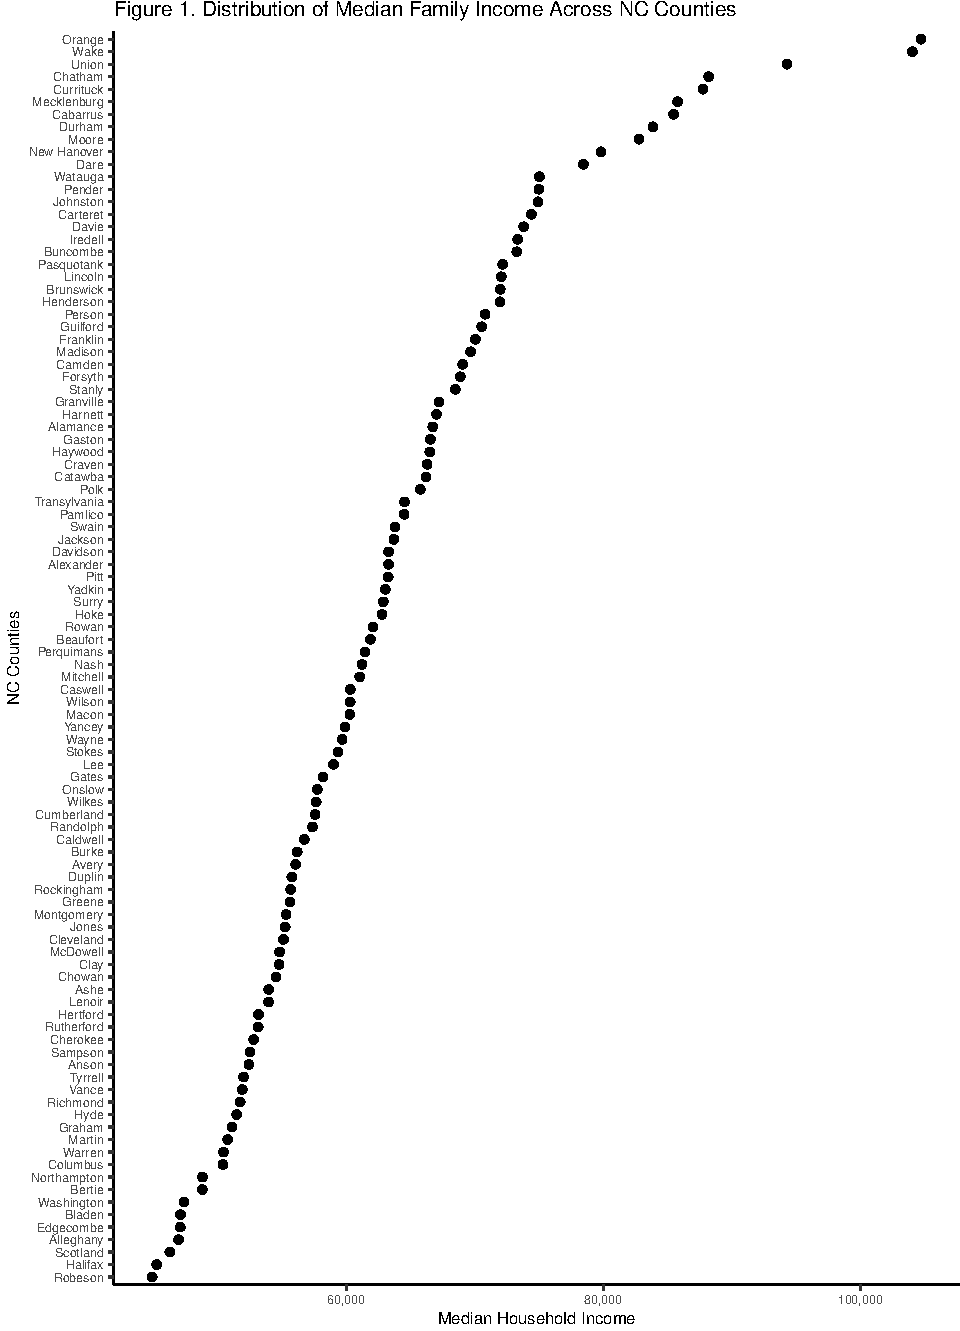
\includegraphics{Project_files/figure-latex/unnamed-chunk-1-1.pdf}
\caption{Median Household Income, NC}
\end{figure}

Figure 2 shows the different types of generators across North Carolina,
defined by fuel type. The counties are coded based on the median family
income in that county. Note that there does appear to be some overlap
between generator location and lower income counties, however a clear
pattern is not discernible based on this visual alone. Energy generators
are diverse in type and widespread throughout the state. Also of note is
that generators powered by solar appear to be the most abundant, despite
widespread knowledge that the predominant energy sources in the US are
fossil fuels.

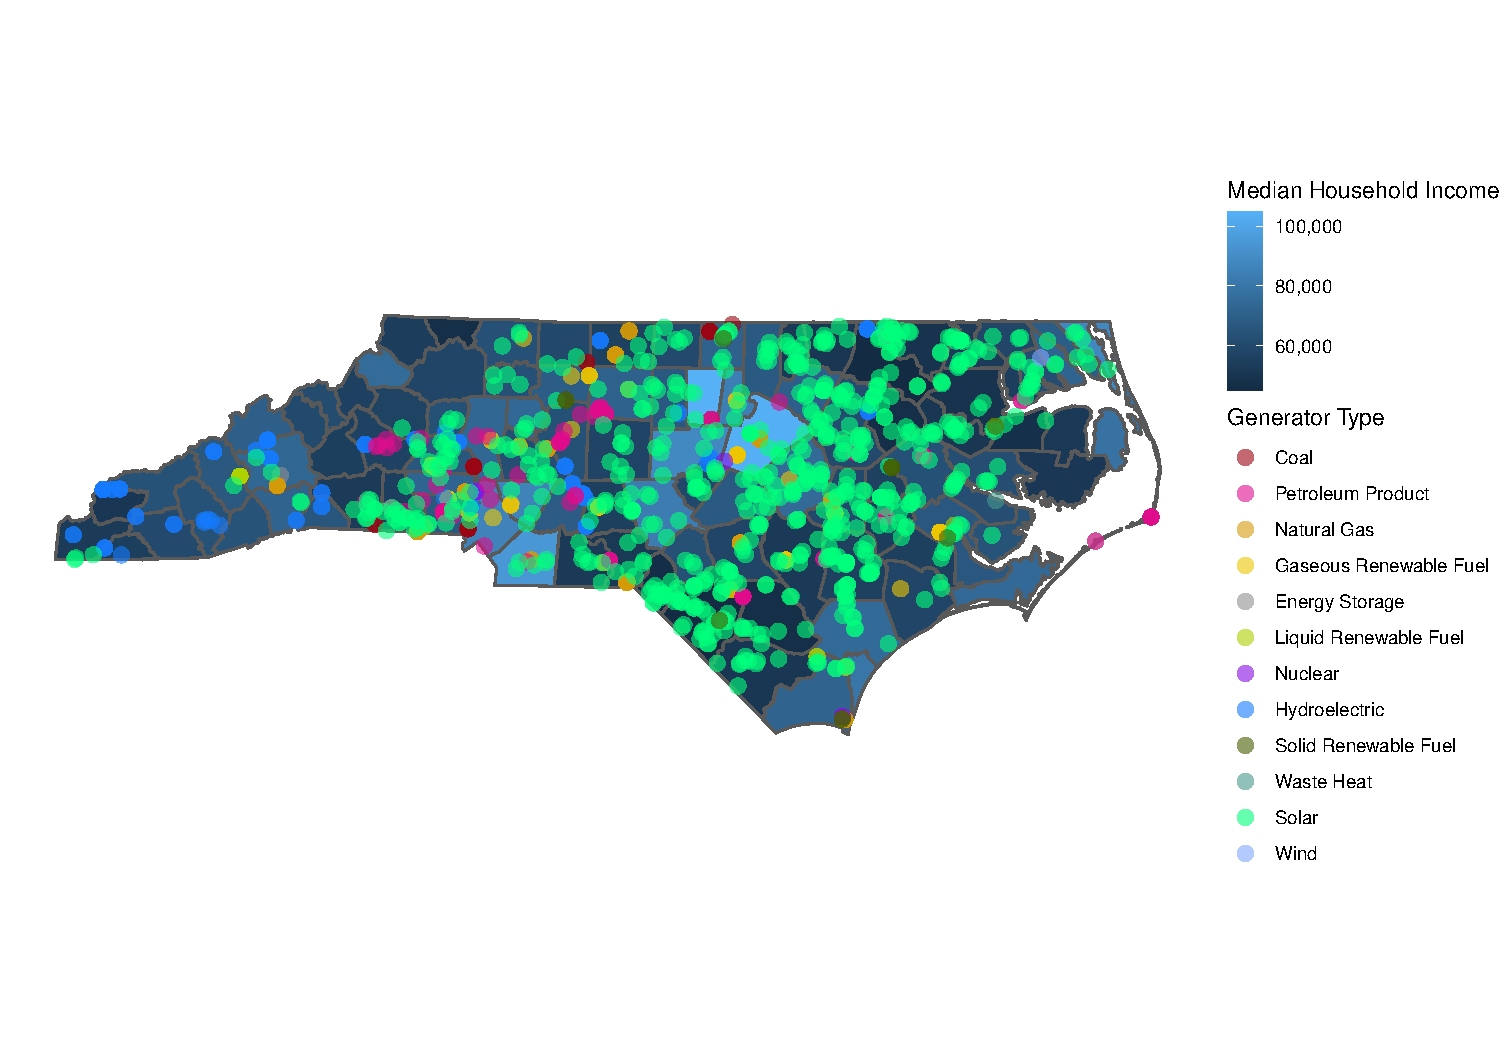
\includegraphics{Project_files/figure-latex/unnamed-chunk-2-1.pdf}

Figures 3 and 4 provide the context for interpreting the above figure.
Figure 3 provides a breakdown of the number of individual generators
based on fuel type, coded according to whether or not that fuel type is
considered a renewable fuel, a fossil fuel, or other, for the state of
North Carolina. While the renewable-fueled generators are far greater in
number, Figure 4 shows that the majority of energy production comes from
fossil fuel sources.

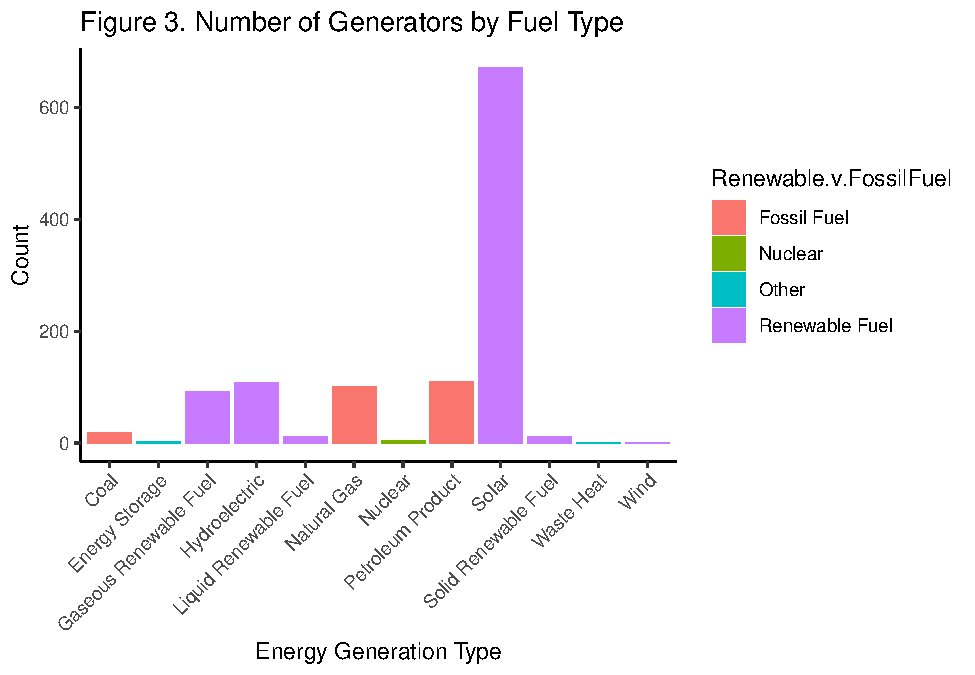
\includegraphics{Project_files/figure-latex/unnamed-chunk-3-1.pdf}

Figure 4 provides a visual representation of the aggregated energy
production potential of the individual generators, using the nameplate
capacity for each generator, again based on fuel type and coded
according to renewable versus fossil fuel categorization. This shows
that the largest contributor to energy production in North Carolina is
natural gas, followed by coal.

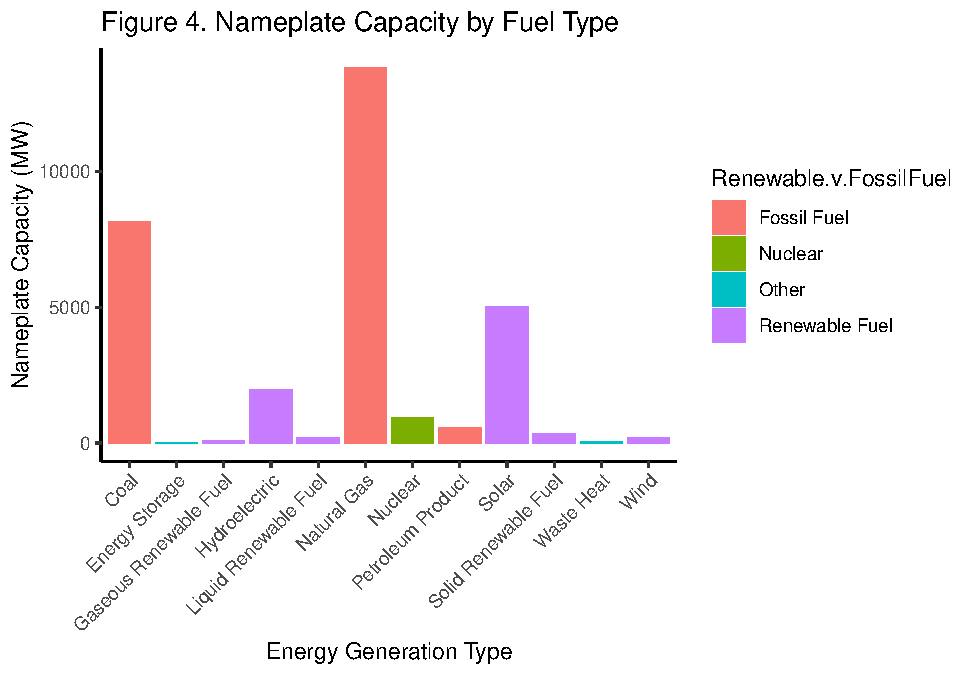
\includegraphics{Project_files/figure-latex/unnamed-chunk-4-1.pdf}

\newpage

\hypertarget{analysis}{%
\section{Analysis}\label{analysis}}

<<<<<<< HEAD
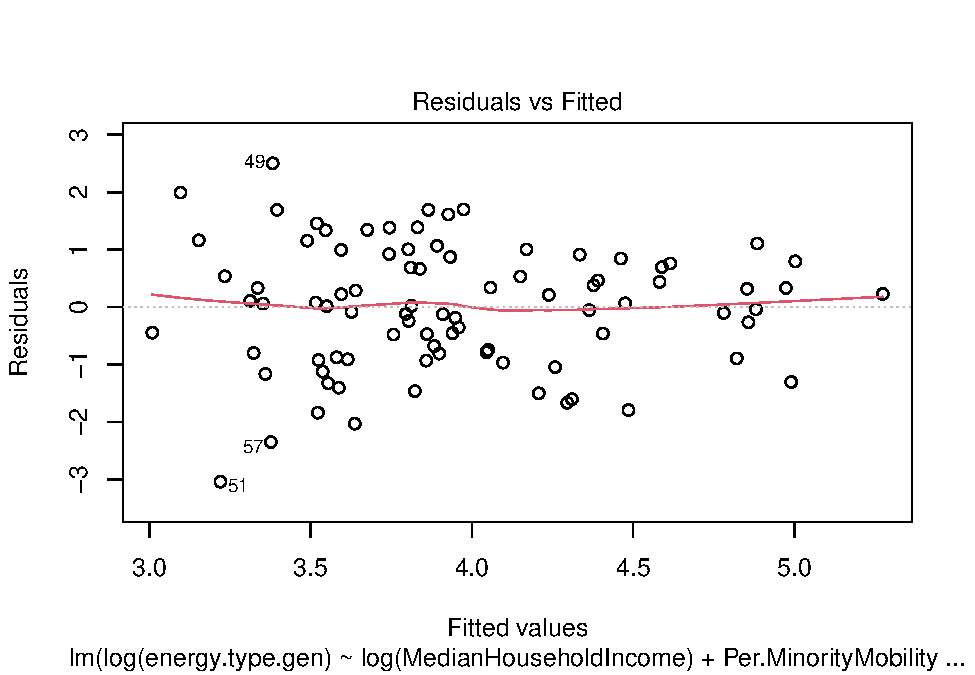
\includegraphics{Project_files/figure-latex/unnamed-chunk-6-1.pdf}
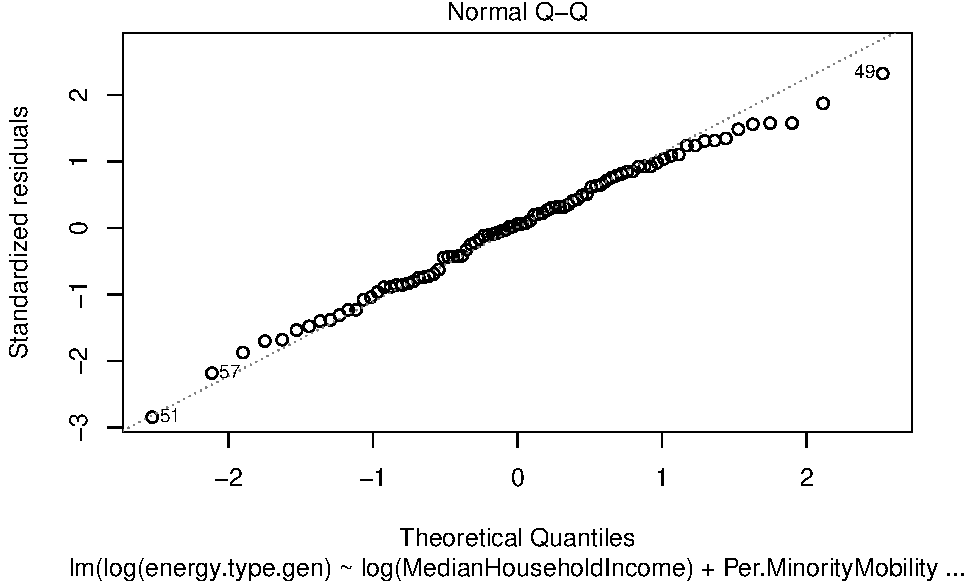
\includegraphics{Project_files/figure-latex/unnamed-chunk-6-2.pdf}
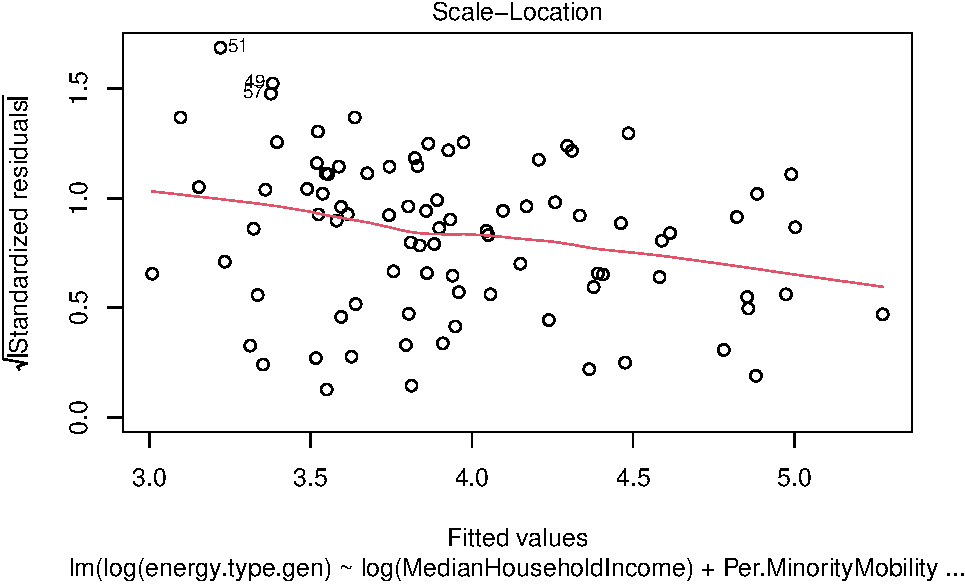
\includegraphics{Project_files/figure-latex/unnamed-chunk-6-3.pdf}
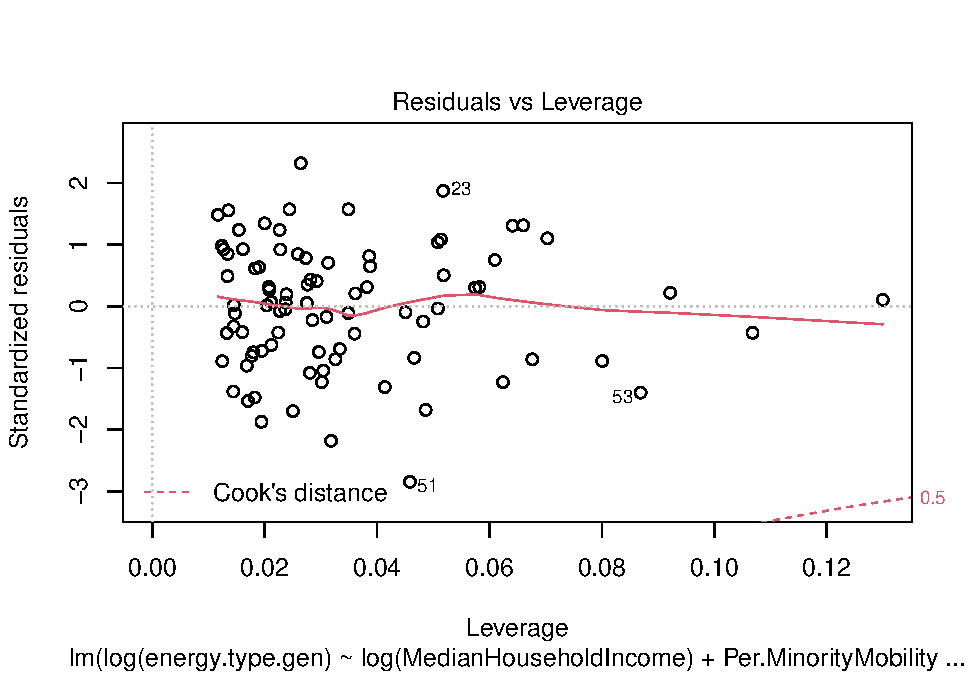
\includegraphics{Project_files/figure-latex/unnamed-chunk-6-4.pdf}

=======
>>>>>>> 0fdb167c805a0a62a4b7d2d1c3c19be3db40f22d
For this analysis we used the generation site's nameplate capacity as
the independent variable demonstrating the size, and assumed impact, to
a community. We aggregated these values into three broad categories:
fossil fuel, renewable, and total energy generation in each county. We
then combined this data with demographic data from the US Census Bureau
for the year 2020. These dependent variables include the county's median
income, the percent of the county's total population that have received
a college or associates degree, and the mobility of the population based
on race and poverty status.

Given that both total energy generation within a county and their median
income are positively skewed, we used log transformation on those
variables. The remaining dependent variables were not log transformed as
we already converted them to percentages of each county's total
population.

To help narrow the focus of our analysis we utilized Akaike's
Information Criterion (AIC) to select our variables for each regression.
This exploratory analysis demonstrated that, given our data limitations,
focusing on renewable data and using our minority mobility and median
income variables will offer the best analysis (AIC=21.31).

The regression analysis (Adj. R-squared = 0.1638) demonstrates with a
1\% increase in a county's renewable energy infrastructure, the county's
median income decreases by 1.51\% (p-value = 0.0329) and the ratio of
population that is a minority increases by 1.97\% (p-value = 0.0117).
This is in line with what we hypothesized, because although renewable
energy is often thought of as a luxury resource, the infrastructure
still undergoes NIMBY criticism by many wealthier individuals.

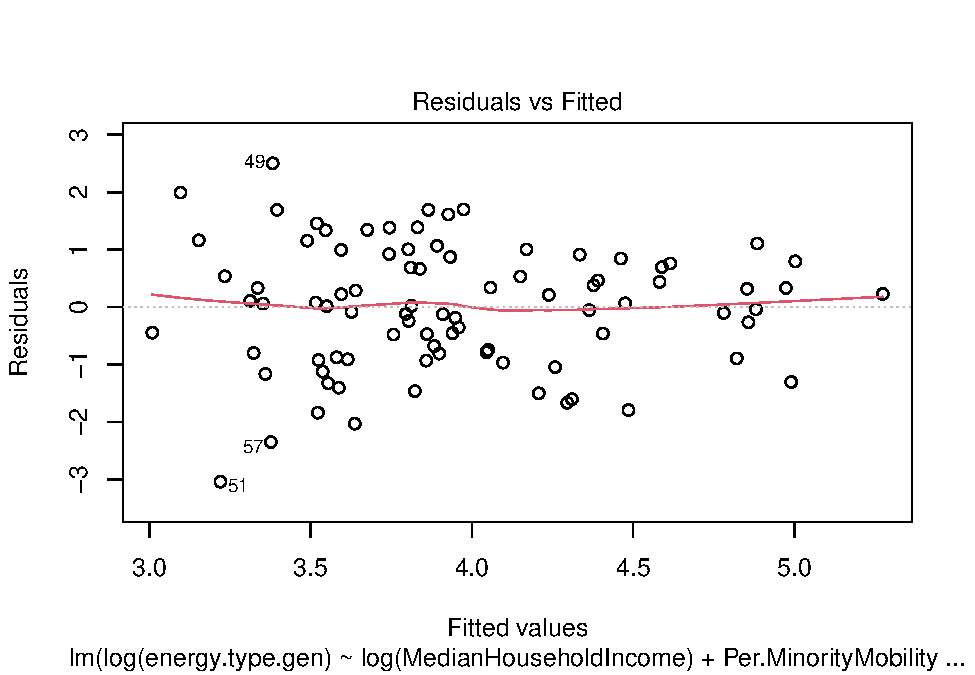
\includegraphics{Project_files/figure-latex/unnamed-chunk-6-1.pdf}
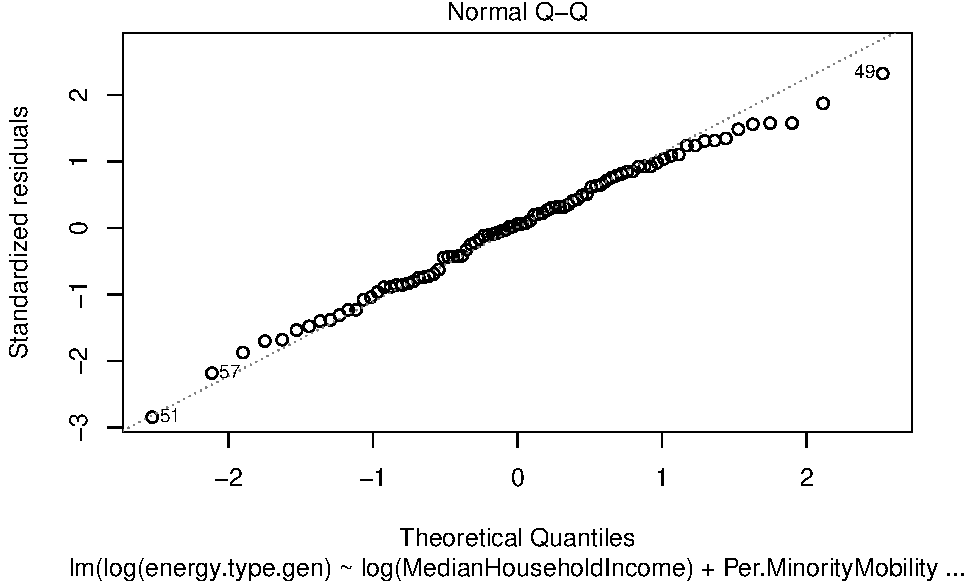
\includegraphics{Project_files/figure-latex/unnamed-chunk-6-2.pdf}
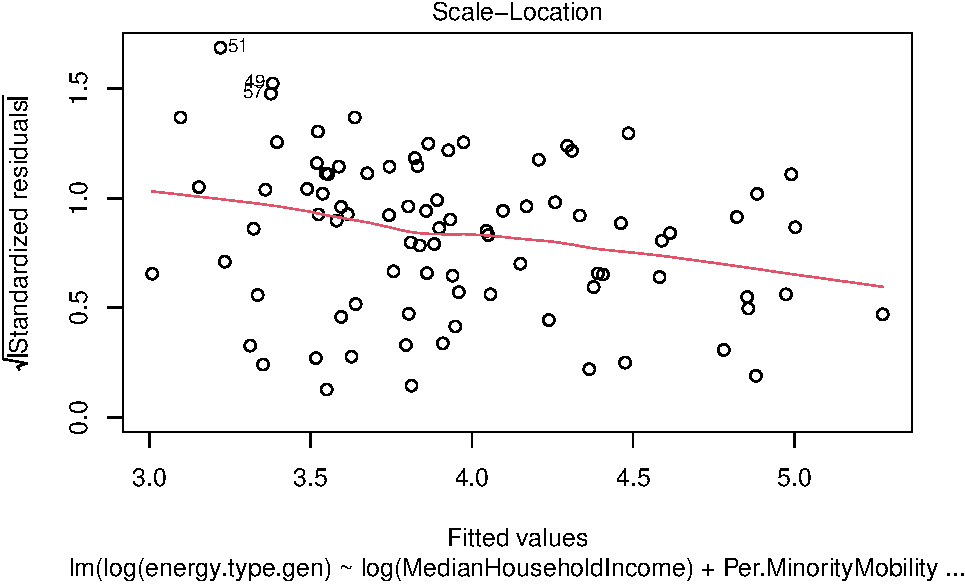
\includegraphics{Project_files/figure-latex/unnamed-chunk-6-3.pdf}
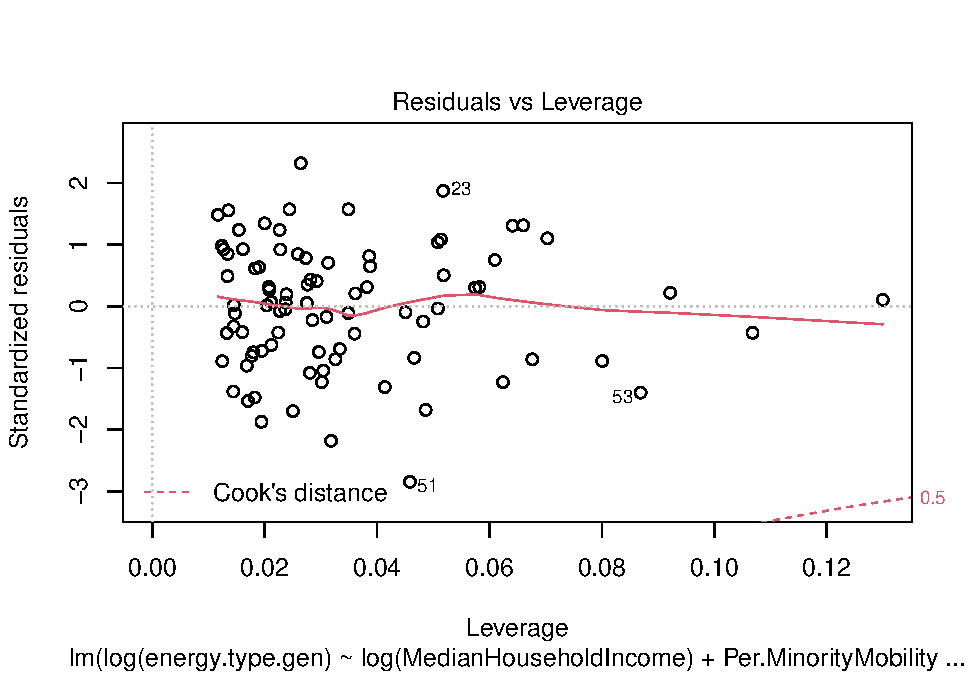
\includegraphics{Project_files/figure-latex/unnamed-chunk-6-4.pdf}

\newpage

\hypertarget{summary-and-conclusions}{%
\section{Summary and Conclusions}\label{summary-and-conclusions}}

\hypertarget{summary}{%
\subsection{Summary}\label{summary}}

In summary, we evaluated the current state of energy generation-related
environmental injustices by investigating the distribution of energy
generators in North Carolina. We found that spatial distributions of
energy generators at the county level showed little correlation with
county-wide demographics. The only correlation significance was found to
be among the spatial distribution of only renewable energy generators
and the demographic variables, median income and the percent minority.
This is likely due to the fact that there are a greater number of
renewable energy sources than fossil fuel sources and correlation cannot
be traced at the county level. Additionally, given that such a small
number of generators are responsible for providing such a large
percentage of the energy needs of the state, a country-wide analysis of
energy generators in relation to low income, minority communities might
return more significant correlations. Despite this, it is still
significant to note that the siting of these renewable energy generators
is correlated with low income, colored communities as this suggests that
even though there is growing awareness around environmental justice,
newer energy sources, albeit renewable, are still being sited near these
historically under-served communities. This shows that we could be on a
path to reproducing the same distributional impacts of energy generation
even though we are transitioning to cleaner energy.

\hypertarget{conclusion}{%
\subsection{Conclusion}\label{conclusion}}

Energy generators have historically and continue to be
disproportionately located next to low income, colored, and under-served
communities. We suggest further assessment of the health and social
implications of siting clean energy generators near under-served
communities. Additionally, a more granular analysis of the communities
immediately surrounding specific plants could reveal correlations not
captured in this county-wide analysis. Further investigation into these
correlations and research around the current siting policies for new
energy generators could shed light on opportunities to prevent the
exacerbation of environmental injustices as our nation's energy
portfolio evolves to embrace renewables.

\newpage

\hypertarget{references}{%
\section{References}\label{references}}

\textless add references here if relevant, otherwise delete this
section\textgreater{}

\end{document}
